\documentclass[a4paper, 12pt, twoside, openright]{mythesis}

\renewcommand{\baselinestretch}{1}       % for squeezing the draft into the page limit, do not use

% Note
% Use \textsc{Name} to separate images, videos, dataset names from the main texts.

% =============================================================================
% Commonly used packages
% =============================================================================

% For removing Package ifpdf Error
%%%%%%\let\ifpdf\relax

% For removing LaTeX Font Warning
\usepackage{lmodern}

% Add Reference in Contents
\usepackage[nottoc]{tocbibind}

% Figures
%\usepackage{subcaption}
\usepackage{float}
%\usepackage[justification=raggedright]{caption}	% makes captions ragged right - thanks to Bryce Lobdell
\usepackage{lscape} % Useful for wide tables or figures.
\usepackage{makecell}
\usepackage{sidecap}

\graphicspath{{figures}{example}}

% Algorithm
\usepackage[lined,ruled,linesnumbered]{algorithm2e}
\usepackage{algorithmic}

% Table and list
\usepackage{booktabs} % Publication quality tables
\usepackage{multirow}
\usepackage{rotating} % sideways
\newcommand{\vergap}[1]{\renewcommand{\arraystretch}{#1}}
\newcommand{\horgap}[1]{\setlength{\tabcolsep}{#1}}
%\specialrule{width}{abovespace}{belowspace}
\newcommand{\dtoprule}{\specialrule{2pt}{0pt}{2pt}}
\newcommand{\dbottomrule}{\specialrule{2pt}{0pt}{\belowrulesep}}
\usepackage{colortbl}

\usepackage{paralist}
\usepackage{enumitem}

% Math
\usepackage{bm} % Make bold, italic math symbols
\usepackage{epsfig} % for figures
\usepackage{graphicx} % another package that works for figures
\usepackage{times}
%\usepackage{mathptmx}
\usepackage{mathtools}
\usepackage{textcomp, gensymb} % math symbol
\usepackage{amssymb,amsmath,amsfonts} % Short math guide for LaTeX ftp://ftp.ams.org/pub/tex/doc/amsmath/short-math-guide.pdf
\usepackage{siunitx} % SI units
\newcommand{\norm}[1]{\left\lVert#1\right\rVert}
\newcommand{\cp}[1]{\left[#1\right]_{\times}}

% Fonts
\usepackage{units}
\usepackage{color}

% Comments
\usepackage{comment}

% Hyperlinks
\usepackage{url} % Hyphenation of URLs.
\usepackage{xcolor}
\usepackage[backref=page]{hyperref}
\hypersetup{colorlinks,breaklinks,
            urlcolor=[rgb]{0.918,0,0.545},
            linkcolor=[rgb]{0.710,0.180,0.141},
            citecolor=[rgb]{0,0.545,0.447}}
\usepackage{bookmark}
%\usepackage[pagebackref=true,breaklinks=true,colorlinks,bookmarks=false]{hyperref} % remove letterpaper=true,
%
\usepackage{slashbox}
\usepackage{xspace}
%\usepackage[table,caption=false]{xcolor}
%\usepackage{setspace}

% Better hyphenation
\usepackage{microtype}

% Appendix
\usepackage[toc,page]{appendix}

% =========================================
% Useful macros
% =========================================

% Latin abbreviations
\newcommand{\etal}{\textit{et al}.~} % ``and others'', ``and co-workers''
\newcommand{\eg}{e.g.,~} % ``for example''
\newcommand{\ie}{i.e.,~} % ``that is'', ``in other words''
\newcommand{\suchthat}{\, \mid \,}

% Math related
\DeclareMathOperator*{\argmin}{\arg\!\min}
\DeclareMathOperator*{\argmax}{\arg\!\max}
\DeclareMathOperator{\avg}{avg}
\DeclareMathOperator{\Tr}{Tr}

% Paragraph
\let\originalparagraph\paragraph
\renewcommand{\paragraph}[2][.]{\originalparagraph{#2#1}}

% Consistent margin adjustment for paragraphs, figures, and sections
\newlength\paramargin
\newlength\figmargin
\newlength\secmargin

\setlength{\secmargin}{0.0mm}
\setlength{\paramargin}{0.0mm}
\setlength{\figmargin}{0.0mm}

% References for figures, tables, equations, chapters, and sections
\newcommand{\chref}[1]{Chapter~\ref{ch:#1}}
\newcommand{\secref}[1]{Section~\ref{sec:#1}}
\newcommand{\figref}[1]{Figure~\ref{fig:#1}}
\newcommand{\tabref}[1]{Table~\ref{tab:#1}}
\newcommand{\eqnref}[1]{\eqref{eq:#1}}
\newcommand{\thmref}[1]{Theorem~\ref{#1}}
\newcommand{\prgref}[1]{Program~\ref{#1}}
\newcommand{\algref}[1]{Algorithm~\ref{#1}}
\newcommand{\clmref}[1]{Claim~\ref{#1}}
\newcommand{\lemref}[1]{Lemma~\ref{#1}}
\newcommand{\ptyref}[1]{Property~\ref{#1}}

% Comments
\long\def\ignorethis#1{}
\newcommand {\sychien}[1]{{\color{blue}\textbf{Po-Chen: }#1}\normalfont}
\newcommand {\coauthorA}[1]{{\color{red}\textbf{Co-author A: }#1}\normalfont}
\newcommand {\coauthorB}[1]{{\color{magenta}\textbf{Co-author B: }#1}\normalfont}
\newcommand {\todo}{{\textbf{\color{red}[TO-DO]\_}}}
\def\newtext#1{\textcolor{blue}{#1}}
\def\modtext#1{\textcolor{red}{#1}}

%\usepackage{ifthen}
%\ifthenelse{\equal{\final}{1}}
%{
%  \renewcommand{\sychien}[1]{}
%}
%{}

\newcommand{\tb}[1]{\textbf{#1}}
\newcommand{\mb}[1]{\mathbf{#1}}
\newcommand{\Paragraph}[1]{\noindent\textbf{#1}}

\newcommand{\jbox}[2]{
  \fbox{%
  	\begin{minipage}{#1}%
  		\hfill\vspace{#2}%
  	\end{minipage}%
  }
}

\newcommand{\jblock}[2]{%
  \begin{minipage}[t]{#1}\vspace{0cm}\centering%
  #2%
  \end{minipage}%
}
	
% Customized definition
\newcommand{\Ic}{\mathcal{I}_{c}}
\newcommand{\It}{\mathcal{I}_{t}}
\newcommand{\Ot}{\mathcal{O}_{t}}
\newcommand{\asin}{\mathrm{asin}}
\newcommand{\acos}{\mathrm{acos}}
\newcommand{\atan}{\mathrm{atan}}
\newcommand{\atanT}{\mathrm{atan2}}
\newcommand{\dotP}{\mathrm{dot}}

\renewcommand{\baselinestretch}{1.5}

%\hypersetup{
%    colorlinks=true,       % false: boxed links; true: colored links
%    linkcolor=blue,          % color of internal links
%    citecolor=blue,        % color of links to bibliography
%    filecolor=blue,      % color of file links
%    urlcolor=blue           % color of external links
%}

%------------------------------------
% Thesis boundary Setting
%-------------------------------------

\textwidth      = 137.0mm
\textheight     = 224.0mm
\topmargin      =  -3.0mm
\headheight     =   7.0mm
\headsep        =  10.0mm
\footskip       =   8.0mm
\oddsidemargin  =  10.6mm
\evensidemargin =  10.6mm
\hoffset = -0.2cm
%\overfullrule=5pt%%

\pagenumbering{roman}% \thispagestyle{myheadings}
\setcounter{page}{1}
%\thispagestyle{empty}

\begin{document}
\title{\textbf{Your Thesis Title}}


\author{ \\  \\ \\
{\it Your Name}\\
{\it Advisor: Shao-Yi Chien} \\ \\ \\ \\  \\ \\
{\it Graduate Institute of Electronics Engineering}\\
{\it National Taiwan University} \\
{\it Taipei, Taiwan}\\ }

{\date{May 2018}}

\maketitle

\frontmatter
\chapter{Abstract}
\label{ch:abstract}

\tableofcontents
\listoffigures
\listoftables

%------------------------------------
% Thesis Body -- begin
%------------------------------------

\mainmatter

\chapter{Introduction}
\label{ch:intro}
Hello, World!

\section{Figure}
\label{sec:figure}
We are from Media IC \& System Lab, as shown in~\figref{misl}.\footnote{All the images in the dissertation are used under Creative Commons license}


\begin{figure}
\begin{center}
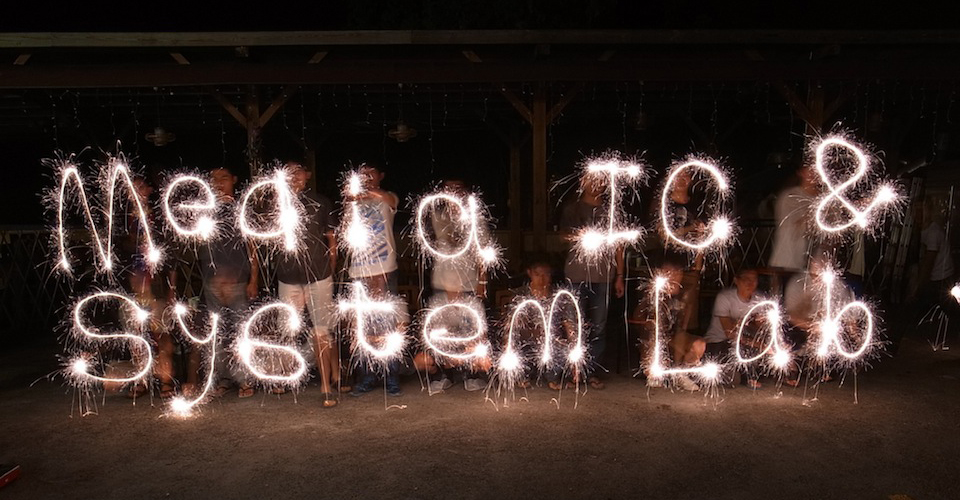
\includegraphics[width=0.8\linewidth]{inc/1_introduction/figure/misl.jpg}
\end{center}
\caption{
We are from Media IC \& System Lab.
}
\label{fig:misl}
\end{figure}


\subsection{Table}
\label{sec:picture}
The related information is shown in~\tabref{lab_information}.

\begin{table}[p]
\vergap{0.8}
\horgap{4.5pt}
\caption{Lab information.}
\vspace{5pt}
\label{tab:lab_information}
\centering
\footnotesize 
\begin{tabular}{cc}
\toprule
Property & Description \\
\midrule
Professor & Shao-Yi Chien \\
Labs & BL421, MD431, MD726 \\
\bottomrule
\end{tabular}
\end{table}

\chapter{Related Work}
\label{ch:related_work}

\section{Repetitive Control and ILC}
\label{sec: Repetitive Control and ILC}


\subsection{Repetitive Control}
\label{sec: Repetitive Control}

\subsection{Iterative Learning Control}
\label{sec: Iterative Learning Control}

  For a SISO, LTI system $G(z)$, which is represented in z-domain and assumed to be asymptotically stable, the ILC learning algorithm can be written in the following form:

\begin{align}
\begin{split}
u_{j+1}(k)& = u_j(k)+L(z)[r(k)-y_j(k)]\\
& = u_j(k)+L(z)e_j(k)
\end{split}
\label{eq:ILClaw}
\end{align}


where $k$ is the time index of the discrete-time signal, the sub-index $j$ represents the $j$th iteration of learning process, $r$ is the trial-invariant reference to be tracked with time interval $N$, $u$ represents the control input of $G(z)$, $y$ is the output of  $G(z)$, $e$ is the tracking error to be reduced, and $L(z)$ is the learning filter to guarantee the stable learning.
 
{$Assumption$ 1.}
Since the z-transform and Fourier transformation of a time sequence is computed over an infinite time interval, all the time signals in this paper are assumed to have infinite length (i.e. $N$$\rightarrow$$\infty$) to meet the requirement of frequency-domain analysis [\cite{silverman1973deconvolution}]. 

$Assumption$ 1 is necessary for ILC analysing in z-domain since the convolution theorem in z-domain is hold iff the time-sequences are all with infinite length.

To analysis the ILC stability condition in frequency domain, the error propagation formula can be obtained from Eq. \ref{eq:ILClaw}:
\begin{equation}
e_{j+1}(k)= [1-L(z)G(z)]e_j(k)
\label{eq:ILCerr}
\end{equation}

By taking Fourier transform of Eq. \ref{eq:ILCerr}, apparently, the tracking error will converge if:
\begin{equation}
\left \| I-G(z)L(z) \right \|_\infty<1
\label{eq:ILCstability}
\end{equation}
where $\left \| \cdot  \right \|_\infty$ denotes $\mathcal{H}_\infty$-norm. It had been proven when the learning filter $L(z)$ satisfies Eq.\ref{eq:ILCstability}, the control input $u_\infty$ and tracking error $e_\infty$ will converge and thus the learning is stable [\cite{norrlof2002time}] . 

{$Remark$ 1.}
To meet the infinite long time signal assumption, the zero-padding technique is applied to extend the reference signal with sufficient long zeros on the both ends to avoid leakage in frequency-domain computation.   


\subsection{Inverse Filter Design of RC and ILC}
\label{sec: Inverse Filter Design of RC and ILC}


\section{Inverse Filter Design Method for Repetitive Control and ILC}

\subsection{Zero Phase Error Tracking Control (ZPETC)}
\label{sec: Zero Phase Error Tracking Control (ZPETC)}

\subsection{Unity Magnitude Error Tracking Control (UMETC)}
\label{sec: Unity Magnitude Error Tracking Control (UMETC)}

\subsection{Direct Inversion Method}
\label{sec: Direct Inversion Method}

\subsection{Iterative Learning of Dynamic Inverse Filters (ILCFF)}
\label{sec: Iterative Learning of Dynamic Inverse Filters (ILCFF)}

\section{Model-free ILC}
\label{sec: Model-free ILC}
To satisfy the stability criteria and the model-free requirement, there are several ways to implement the model-free leaning law. Here the time-reversal based ILC and MFIIC approaches are introduced.



\subsection{Model-free Adjoint-based ILC}
\label{sec: Model-free Adjoint-based ILC}

Consider the adjoint-based ILC [\cite{ye2005zero}; \cite{owens2009robust}], the learning filter $L(z)=\alpha G^{*}(z)$ is chosen with a sufficiently small learning gain $\alpha>0$ to guarantee the stability condition. The reason why the adjoint-based learning filter is capable to stabilize the learning is the phase effect of the system could be cancelled, hence the stable learning can be hold if the learning gain is properly selected.

To realize the adjoint-based learning law:
\begin{equation}
u_{j+1}(k)= u_{j}(k)+ \alpha G^{*}(z)e_{j} (k)
\label{eq:TimeRever}
\end{equation}

the term $\alpha G^{*}(z)e_{j} (k)$ can be obtained by using the reversed time filtering technique as shown in [\cite{ye2005zero}]:

\begin{enumerate}
  \item Reverse the error signal: $e_{j1}(k)=e_{j}(N-k)$;
  \item Feed the reversed error signal to the system: $e_{j2}(k)=G(z)e_{j1}(k)$;
  \item Reverse $e_{j2}(k)$ again, and multiply with $\alpha$:  $e_{j3}(k)= \alpha e_{j2}(N-k)$
  \item Conduct the learning law: $u_{j+1}(k)=u_{j}(k)+e_{j3}(k)$;
\end{enumerate}

For the adjoint-based learning approach, the robustness can be improved compared with the inversion-based approach, especially considering the effect of high frequency model uncertainty [\cite{owens2009robust}]. However, since the convergence rate is limited by the small learning gain, this disadvantage leads to a critical issue of the time-consuming learning process in real application.

\subsection{Model-free Inversion-based Iterative Control (MFIIC)}
\label{sec: Model-free Inversion-based Iterative Control (MFIIC)}

Consider the SISO, LTI and stable system $y_j(k)=G(z)u_j(k)$, the model-free inversion-based learning law can be written as: 

\begin{align}
U_{j+1}(e^{j\omega})=\begin{cases}
 & U_{j}(e^{j\omega})+\rho_j\frac{U_j(e^{j\omega})}{Y_j(e^{j\omega})}E_j(e^{j\omega}),\\ 
 &\text{ if } Y_j(e^{j\omega})\neq 0 $ and $ R(e^{j\omega})\neq 0 ;\\ 
 & U_{j}(e^{j\omega});\text{ otherwise}
\end{cases}
\end{align}

where $U_j(e^{j\omega})$ and $Y_j(e^{j\omega})$ is the frequency-domain representation of $u_j(k)$ and $y_j(k)$ respectively; and the learning gain $\rho_j$ is equal to 1 for MFIIC [\cite{kim2012modeling}] and $\rho_j=f(|Y_j(e^{j\omega})|)$ is a function of $|Y_j(e^{j\omega})|$ for NLIIC [\cite{de2019data}] to improve the robustness. 

For this approach, the updating computation in frequency-domain is relative simple and time-efficient compared to the reversed time filtering approach. Moreover, since the estimated learning filter is inversion-based, the learning will converge after few iterations. However, due to the learning filter is constructed by measured data, while the unpredicted disturbances dominate the output signal, the updated control input may be dramatically amplified in some frequency components. This observation had been indicated in [\cite{de2018improving}]. Moreover, since the noisy learning filter is conducted iteration by iteration over the whole learning process, while the adaptive learning gain is introduced [\cite{de2019data}], the tracking performance in steady-state is limited. 

\subsection{Non-Linear Inversion-based Iterative Control (NLIIC)}
\label{sec: Non-Linear Inversion-based Iterative Control (NLIIC)}

\subsection{Comparison of existed model-free ILC}
\label{sec: Comparison of existed model-free ILC}

In this paper. we propose a novel method to remedy the difficulties for the model-free ILC mentioned above. Specifically, the proposed method is expected to
\begin{enumerate}
  \item Improve the learning transient against output disturbances;
  \item Achieve lower tracking error in steady-state.
\end{enumerate}

%------------------------------------
% Thesis Body -- end
%------------------------------------

\bibliographystyle{IEEEtran}
\bibliography{thesis}
\end{document}
